\documentclass[11pt,a4paper,oneside]{article}

\usepackage{a4wide}
\usepackage{graphicx}
\usepackage{hyperref}
\usepackage{listings}
\usepackage[usenames,dvipsnames]{color}

\newcommand{\red}[1]{\textcolor{red}{#1}}
\newcommand{\blue}[1]{\textcolor{blue}{#1}}
\newcommand{\green}[1]{\textcolor{ForestGreen}{#1}}
\newcommand{\orange}[1]{\textcolor{Orange}{#1}}
\newcommand{\nid}{\noindent}

\begin{document}
\title{RDSL: Robot Domain Specific Language (DSL1)\\ {\Large(work-in-progress)}}


\author{E. Jans, H. Bruyninckx}
\date{\today}
\maketitle

\section{Overview}
\label{sec:overview}

The \textbf{RDSL} (DSL1) can be used to describes a sepcific robot
completely by it's kinematic chain. The kinematic chain contains
different sub models and resolutions so a great deal of flexibility
(modularity) is available. The modelling language(\textit{metametamodel})
is xml\footnote{\url{http://en.wikipedia.org/wiki/Xml}} with xsd schema
\textit{metamodels}.

\begin{figure}[h]
  \centering
  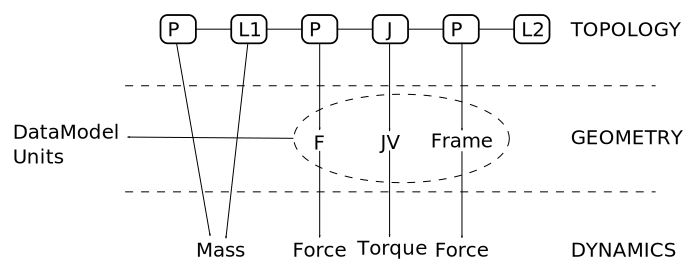
\includegraphics[width=1\columnwidth]{figs/RDSL_Layers}
  \caption{Levels of RDSL}
  \label{fig:rdsl-sketch}
\end{figure}

We can divide the dsl into three sub models each adding more information to the
kinematic chain.
 
\subsection{Topology}
\label{sub:topology}

This submodel describes the basic joints and links of a robot and it's connections
with the port primitive from the hierarchical hypergraph metamodel\footnote{LinkToHH}.

\subsection{Geometry}
\label{sub:geometry}

This submodel adds frames, joint values, data models and units to the chain. The
geometry is based on the Geometric semantics\footnote{LinkToGemSem} model.

\subsection{Dynamics}
\label{sub:dynamics}

The frames and joint values of the geometry model will have mass, forces and
torque when dynamics are added.

\end{document}
